\documentclass[french,a4paper,10pt,twocolumn]{article}
\usepackage{graphicx} % Required for inserting images
\usepackage{graphicx} % Required for inserting images
\usepackage[style=authoryear, backend=biber]{biblatex}
\usepackage[left=1cm,right=1cm,top=1cm,bottom=2cm]{geometry}
\usepackage[style=authoryear, backend=biber]{biblatex}
\usepackage{hyperref}
\usepackage{csquotes}
\usepackage{animate}
\usepackage[T1]{fontenc}
\usepackage{amsmath}
\usepackage[french]{babel}

\title{PRO3600: Mars Lander}
\author{Augustin Bresset | Zacharie March}
\date{January 2024}
\addbibresource{references.bib} %Imports bibliography file

\begin{document}
\onecolumn
\maketitle

\begin{figure}[h]
    \centering
    
\includegraphics[scale=0.2]{images/logo-tsp-fond-blanc.png}
    \caption{Logo TSP}\label{fig:logo}
\end{figure}

\tableofcontents
\twocolumn
\pagebreak

\section{Introduction}

\subsection{Présentation du problème: Mars Lander}

Mars Lander est un problème d'optimisation proposé sur la plateforme \cite[]{codingame_mars_lander}.
Ce jeu consiste en le contrôle d'un vaisseau spatial et de ses caractéristiques (position, vitesse, puissance des moteurs, angles de rotation…) 
afin de le faire atterrir en toute sécurité et en douceur sur Mars sur une surface plane, quelle que soit sa position de départ. 
L'idée est donc de trouver une trajectoire fonctionnelle.

\subsubsection{Environnement}

La surface de Mars est représenté localement par une suite continue de segments.
Parmis ces segments un et un seul est rigouresement vertical, celui-ci définit la zone d'atterissage que la navette doit viser.
\begin{figure}[h]
    \centering
    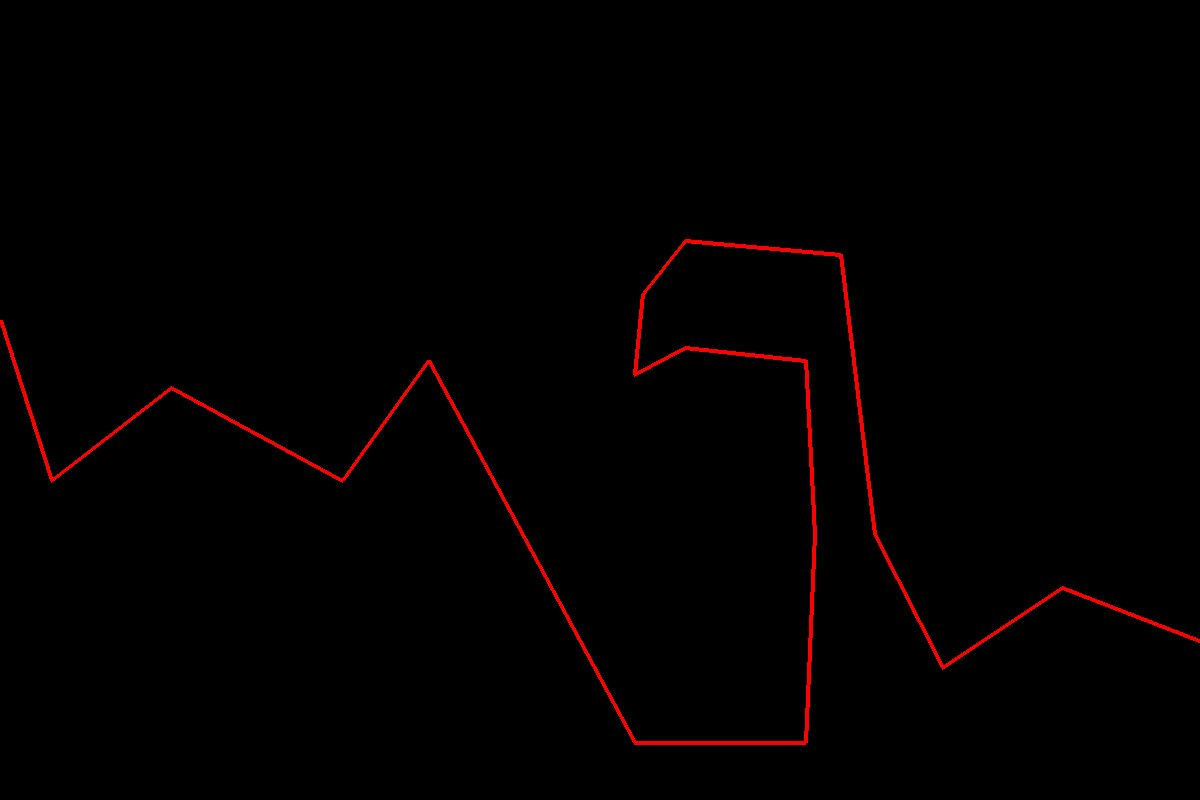
\includegraphics[scale=0.2]{images/cave_map.jpeg}
    \caption{Exemple de carte du problème}\label{fig:map}
\end{figure}

\subsubsection{Espace des Etats}

L'état du vaisseau est représenté par un vecteur de 7 valeurs:
\begin{itemize}
    \item $x$: position horizontale
    \item $y$: position verticale
    \item $hSpeed$: vitesse horizontale
    \item $vSpeed$: vitesse verticale
    \item $fuel$: quantité de carburant restante
    \item $rotate$: angle de rotation
    \item $power$: puissance des moteurs
\end{itemize}
Certains de ces paramètres est borné par une valeur minimale et maximale que voici: 

\begin{itemize}
    \item $x$: $[0, 7000]$
    \item $y$: $[0, 3000]$
    \item $fuel$: $ [0, \infty [ $ 
    \item $rotate$: $[-90, 90]$
    \item $power$: $[0, 4]$
\end{itemize}

\subsubsection{Espace des Actions}

Toutes les secondes, en fonction des paramètres d’entrée (position, vitesse, fuel, etc.), 
le programme doit fournir le nouvel angle de rotation souhaité ainsi que la nouvelle puissance des fusées de Mars Lander.
Mais les commandes de puissance des fusées et de l’angle de rotation sont bornés par les valeurs suivantes qui forme l'espace des actions:
\begin{itemize}
    \item rotation: $[-15, 15]$ 
    \item puissance: $[-1, 1]$
\end{itemize}

\subsubsection{Conditions d'atterrissage}

Les conditions d'atterissage doivent être représentées:
\begin{itemize}
    \item atterrir sur un terrain plat
    \item atterrir en position verticale (angle d'inclinaison = 0°)
    \item la vitesse verticale doit être limitée ($\le 40m.s^{-1}$ en valeur absolue)
    \item la vitesse horizontale doit être limitée ($\le 20m.s^{-1}$ en valeur absolue)
\end{itemize}

\subsubsection{Algorithme Génétique}

Les algorithmes génétiques sont des algorithmes d'optimisation stochastique inspirés de la théorie de l'évolution naturelle.
Ils sont basés sur le principe de \textbf{sélection naturelle}.\\
Dans un premier temps on génère une \textbf{population} de solution aléatoire, puis on évalue la qualité de chaque solution.
On sélectionne fait ensuite évoluer cette population à travers des phénomènes semblables à la sélection naturelle tel que la \textbf{sélection}, la \textbf{reproduction} et la \textbf{mutation}.
On répète ce processus jusqu'à ce qu'une solution satisfaisante soit trouvée.
Dans notre problème, une solution est définie par une trajectoire, c'est à dire une suite de commande à effectuer par le vaisseau.\\
L'évolution d'une population de solution se fait donc en plusieurs étapes:
\begin{itemize}
    \item \textbf{Sélection}: On sélectionne les meilleurs solutions de la population
    \item \textbf{Reproduction}: On fait se reproduire des solutions choisies aléatoirement
    \item \textbf{Mutation}: On applique une mutation à la nouvelle génération afin d'explorer de nouveaux espaces
\end{itemize}
Le calcul du score peut dépendre de nombreux paramètres, dans notre cas on a choisi de prendre en compte les paramètres suivants:
\begin{itemize}
    \item La \textbf{distance} au sol qui sépare la zone de collision et d'atterissage
    \item Les \textbf{vitesses} verticale et horizontale 
    \item L'\textbf{angle} d'inclinaison du vaisseau à l'atterissage
\end{itemize}


\subsection{Objectif}

Notre objectif est de résoudre ce problème à l'aide d'une approche heuristique, les algorithmes génétiques. 
Pour cela on à définit plusieurs points afin de mener à bien notre projet: 
\begin{itemize}
    \item Création d'une \textbf{interface graphique} sur pygame
    \item Mise en place d'une \textbf{interface client} permettant de piloter la navette
    \item Calcul de \textbf{solution} notamment à l'aide d'algorithme génétique    
\end{itemize}

\subsubsection{Cahier des charges}

Développer une applicattion avec interface graphique. Les fonctionnalités attendues sur l'application sont les suivantes:
\begin{itemize}
    \item Choix de la solution à utiliser
    \item Choix de la carte à utiliser
    \item Exécution de la simulation
    \item Adapter l'affichage en fonction de la solution
\end{itemize}

\subsection{Organisation du projet}

\subsubsection{Répartition des tâches}

En claire la répartition des tâches est la suivante:
\begin{itemize}
    \item \textbf{Augustin Bresset}\\
        Développement de l'environnement et des solutions 
    \item \textbf{Zacharie March}\\
        Développement de l'interface graphique et de l'interface client
\end{itemize}
Dans les deux cas, un apprentissage de la librairie pygame est nécessaire. Que ce soit pour la création de la solution "manuelle" (contrôle par l'utilisateur)
ou pour la création de l'interface graphique.

\subsubsection{Outils de travail}

Afin de communiquer, nous nous reposons pour la communication active sur plusieurs outils, étant deux,
nous n'étions pas restreint par le besoin de créer un groupe sur un outil de communication.
Pour la commun passive nous avons créée une organization sur Github dans laquelle on peut trouver deux repertoire:
\begin{itemize}
    \item \textbf{backend}: Contient le code source du projet
    \item \textbf{meta}: Contient la documentation du projet (et ce livrable)
\end{itemize}

\subsubsection{Organisation du code}

Afin de faciliter la lecture du code ainsi que le développement, nous avons séparer en plusieurs modules le code source:
\begin{itemize}
    \item \textbf{environment}: Contient le code source de l'environnement
    \item \textbf{gui}: Contient le code source de l'interface graphique
    \item \textbf{solution}: Contient le code source des solutions
    \item \textbf{utils}: Contient le code source des fonctions utilitaires
\end{itemize}



\section{Développement}



\subsection{Architecture du projet}

\subsubsection{Environnement}

L'environnement est composé de plusieurs classes:
\begin{itemize}
    \item \textbf{Environment}: Classe principale de l'environnement, elle permet de gérer les interactions entre les entités et l'environnement
    \item \textbf{Surface}: Classe permettant de gérer la surface de Mars
    \item \textbf{Lander}: Classe permettant de gérer le vaisseau
    \item \textbf{Action}: Classe permettant de gérer les actions du vaisseau
    \item \textbf{Utils}: Classe permettant de gérer les constantes et les fonctions utilitaires
    \item \textbf{Entity}: Classe abstraite permettant de gérer les entités
    \item \textbf{Constants}: Classe permettant de gérer les constantes
\end{itemize}

\subsubsection{Gui}

\subsubsection{Solution}    

Une solution est définie par une classe abstraite \textbf{AbstractSolution} qui permet de définir les méthodes communes à toutes les solutions.
On a ensuite deux types de solutions:
\begin{itemize}
    \item \textbf{ManualSolution}: Solution manuelle permettant de piloter le vaisseau à l'aide du clavier
    \item \textbf{GeneticSolution}: Solution génétique permettant de piloter le vaisseau à l'aide d'un algorithme génétique
\end{itemize}



\pagebreak
\printbibliography
\end{document}
